\section{Descrizione proposta di stage}
\label{sez:descrizione-stage}

L'idea alla base dello \textit{stage} è quella di automatizzare la creazione di un documento denominato *allegato tecnico*.\\  
Questo documento raccoglie tutte le informazioni tecniche relative a un progetto software, comprese le tecnologie utilizzate,
la struttura del progetto, le scelte architetturali ed il piano di \textit{testing}, per citare alcune delle sezioni.\\  
Fino ad oggi, l'azienda ha sempre realizzato questo documento manualmente. Tuttavia, con l'aumento dei progetti e delle risorse impiegate,
l'introduzione di un \textit{tool} per automatizzare, anche solo parzialmente, questo processo risulta particolarmente interessante.\\  

\noindent L'obiettivo dello \textit{stage} è quindi la realizzazione di una piattaforma \textit{web} che, tramite l'uso di sistemi di \gls{ai-generativa},\\  
permetta di generare automaticamente questo documento.\\  
L'utente finale della piattaforma sarà un membro del \textit{team} di sviluppo o il \textit{project-manager}.\\  
Questi avrà la possibilità di compilare dei \textit{Preset}, ovvero una serie di domande progettate \textit{ad hoc}
per raccogliere le informazioni necessarie alla creazione del documento, ottimizzate in base al tipo di progetto da sviluppare (ad esempio, una \textit{Web App} o una \textit{Mobile App}).\\  
Il sistema utilizzerà i servizi di \gls{ai-generativa} forniti da AWS (AGGIUNGERE TERMINE GLOSSARIO) per creare il documento automaticamente.\\  

\noindent Inoltre, l'utente avrà la possibilità di rigenerare il documento, in parte o nella sua totalità, inserendo un \gls{prompt}.\\  
Questo \gls{prompt} sarà una frase o un paragrafo che guiderà il sistema, consentendo all'utente di specificare le migliorie o modifiche da apportare al documento.\\  
Tutte le versioni del documento verranno salvate, permettendo di visualizzare le differenze tra una versione e l'altra.\\  
Una volta soddisfatto del risultato, l'utente potrà scaricare il documento in formato \textit{PDF}.\\  
Nella {\hyperref[fig:project-schema]{Figura 2.1}} è mostrato uno schema che rappresenta l'idea alla base del progetto.\\  


\begin{figure}[H]
    \label{fig:project-schema}
    \centering
    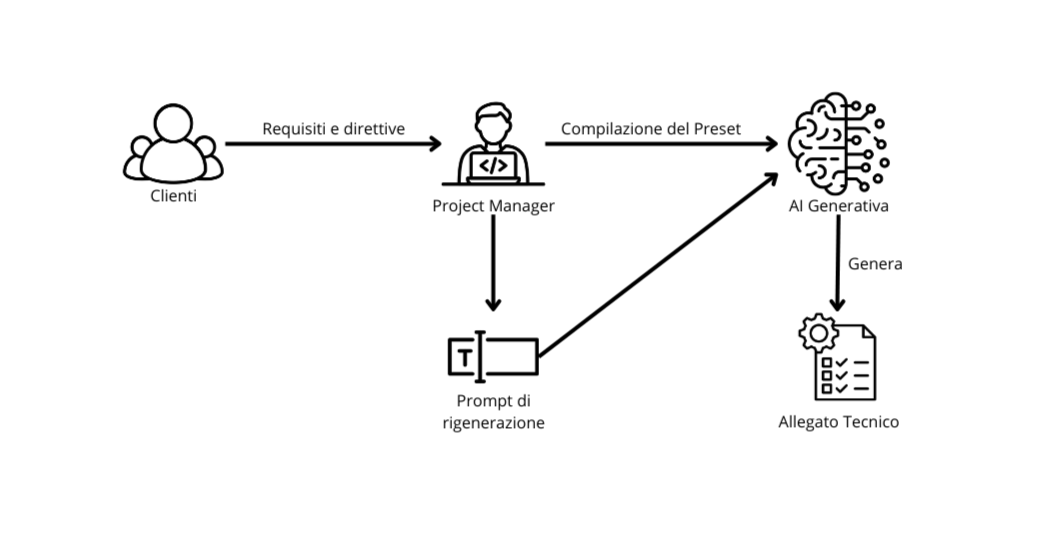
\includegraphics[scale=0.6]{gen-ai-documentation-schema.png}
    \caption{Schema del progetto}
\end{figure}